%%%%%%%%%%%%%%%%%%%%%%%%%%%%%%%%%%%%%%%%%%%%%%%%%%%%%%%%%%%%%%%%%%%%%%%%%%%
% filename    : sp.tex
% author      : 
%%%%%%%%%%%%%%%%%%%%%%%%%%%%%%%%%%%%%%%%%%%%%%%%%%%%%%%%%%%%%%%%%%%%%%%%%%%

% BUGFIX: Save LaTeX kernel version of \@xfloat
\makeatletter
\let\my@xfloat\@xfloat
\makeatother

% use ateneo de naga etd class (actually modified virginia tech's etd class)
\documentclass[oneside]{etd}

% BUGFIX: Create a modified copy of \@xfloat using the kernel definition
\makeatletter
\def\@xfloat#1[#2]{
	\my@xfloat#1[#2]%
	\def\baselinestretch{1}%
	\@normalsize \normalsize
}
\makeatother

% use these packages

\usepackage{graphicx}
\usepackage{amssymb}
\usepackage{gensymb}
\usepackage{latexsym}
\usepackage{amsmath}
%\usepackage[lineno5,noindent]{lgrind}
%\usepackage{rotating} 
%\usepackage{makeidx}
%\usepackage{stmaryrd}
\usepackage{float}
\usepackage{subfigure}
\usepackage{hyperref}
%\usepackage{cite}
%\usepackage{moreverb}
%\usepackage{pictexwd,dcpic}
\usepackage{algorithm,algorithmic}
\renewcommand{\algorithmicrequire}{\textbf{Input:}}
\renewcommand{\algorithmicensure}{\textbf{Output:}}
\usepackage{tikz}
\usetikzlibrary{positioning,calc}

\usepackage{listings}
\definecolor{cppred}{rgb}{0.6,0,0} % for strings
\definecolor{cppgreen}{rgb}{0.25,0.5,0.35} % comments
\definecolor{cpppurple}{rgb}{0.5,0,0.35} % keywords
\definecolor{cppdocblue}{rgb}{0.25,0.35,0.75} % doc
 
\lstset{language=C++,
basicstyle=\linespread{0.8}\ttfamily\small,
keywordstyle=\color{cpppurple}\bfseries,
stringstyle=\color{cppred},
commentstyle=\color{cppgreen},
morecomment=[s][\color{cppdocblue}]{/**}{*/},
numbers=left,
numberstyle=\tiny\color{black},
% stepnumber=2,
numbersep=10pt,
tabsize=4,
showspaces=false,
showstringspaces=false}

\graphicspath{{figures/}{./}}

%\renewcommand{\floatpagefraction}{0.8}

\makeindex

%%%%%%%%%%%%%%%%%%%%%%%%%%%%%%%%%%%%%%%%%%%%%%%%%%%%%%%%%%%%%%%%%%%%%%%%%%%

\title{Parallel Implementation of the A* Pathfinding Algorithm on a Purely-Functional Programming Language}
\author{My Name}
\department{Computer Science}
\BSdegree
\field{Computer Science}
\degreemonth{Month Day}  % date of final defense
\degreeyear{2020}

\fourstudents
{Prince Bernie B. Colis}
{John Kenneth S. Lesaba}
{Jon Ariel N. Maravilla}
{Karl Frederick R. Roldan}

\fourstudentsheader
{Colis, Lesaba, Maravilla, and Roldan}

\fourdegrees
{Computer Science}
{Computer Science}
{Computer Science}
{Computer Science}


\advisor
{Adrian Leo Pajarillo}
\threemembers
{First Panel Member}
{Second Panel Member}
{Third Panel Member}
\deanandchair
{Joshua C. Martinez, MIT}
{Marianne P. Ang, MS}

\keywords{parallel programming, functional programming, graph theory}


\begin{document}

\maketitle
\makerecomm
\makeacceptance
\makedeclaration

%%%%%%%%%%%%%%%%%%%%%%%%%%%%%%%%%%%%%%%%%%%%%%%%%%%%%%%%%%%%%%%%%%%%%%%%%%%
%                    ABSTRACT/EXECUTIVE SUMMARY                           %
%%%%%%%%%%%%%%%%%%%%%%%%%%%%%%%%%%%%%%%%%%%%%%%%%%%%%%%%%%%%%%%%%%%%%%%%%%%

\begin{execsummary}
	To be filled in later. \verb|/*TODO*/|.
\end{execsummary}

	
\begin{dedication}

I dedicate this research work to all of humanity.

\end{dedication}


\begin{acknowledgements}

I thank everyone who helped me finish this thesis.

\end{acknowledgements}


\begingroup
\renewcommand*{\addvspace}[1]{}
\tableofcontents
\listoffigures
\listoftables
\endgroup

\beginbody
\pagenumbering{arabic}

%%%%%%%%%%%%%%%%%%%%%%%%%%%%%%%%%%%%%%%%%%%%%%%%%%%%%%%%%%%%%%%%%%%%%%%%%%%
\chapter{Introduction}
%%%%%%%%%%%%%%%%%%%%%%%%%%%%%%%%%%%%%%%%%%%%%%%%%%%%%%%%%%%%%%%%%%%%%%%%%%%

Functional programming has suddenly risen to popularity 
with examples that include Scala, Clojure, ReactJS, and 
other languages adopting lambda expressions. Reasoning 
about program correctness in a pure function can be done 
in a dependently-typed, proof assistant such as Coq or 
Agda\cite{Breitner2018}\cite{SpectorZabusky2018}\cite{ElBakouny2017}. 
Likewise, pure functions can be easily proved by using 
induction. Composing two proven functions into a single 
function should also give the correct result\cite{AbelBenkeBove2005}.

This research aims to utilize the existing A* pathfinding 
algorithm\cite{ZaghloulAlJami2017}\cite{WeinstockHolladay}
and find a way to develop a reasonably-efficient 
purely functional implementation of the algorithm using parallel 
data structures such as STMs or MVars\cite{Marlow2013}.  
The main objective of the research is 
to find an efficient concurrent implementation of a maze solver 
in a purely functional programming environment with comparable 
performance and space complexity of a performant imperative 
programming language.

% The Shortest Common Superstring (SCS) problem, known to be NP-Complete,
% seeks the shortest string that contains all strings from a given set.
% In this paper, we provide the summary of the problem and some of its characteristics.

% The SCS problem has been extensively studied for its
% applications in string compression and DNA sequence assembly \cite{Ma2009}.

% The superstring problem has applications to data storage,
%  specifically, data (string) compression \cite{Gallant1980}. 
% In many programming languages, a character string may be 
% represented by a pointer to that string. 
% The problem for the compiler is to arrange strings 
% so that they may be ``overlapped'' as much as possible.

% DNA sequence assembly is another  problem to which an SCS algorithm is known to apply.
% The $sequencing$ problem in molecular biology is to ``read'' a string of DNA,
% which can be viewed as a string over the alphabet \{A,C,G,T\}. Sequencing produces such a large number of fragments that
% almost all genome positions are covered by many fragments. This short fragments
% thus have large overlaps between other pieces. Hence, they can be given as an input to SCS algorithm.
% Figure \ref{fig:dna-overlap} shows an overlap graph consisting DNA reads (or fragments) as nodes. 



% \begin{figure*}
% \centering
% \fbox{
% \scalebox{0.65}{
% 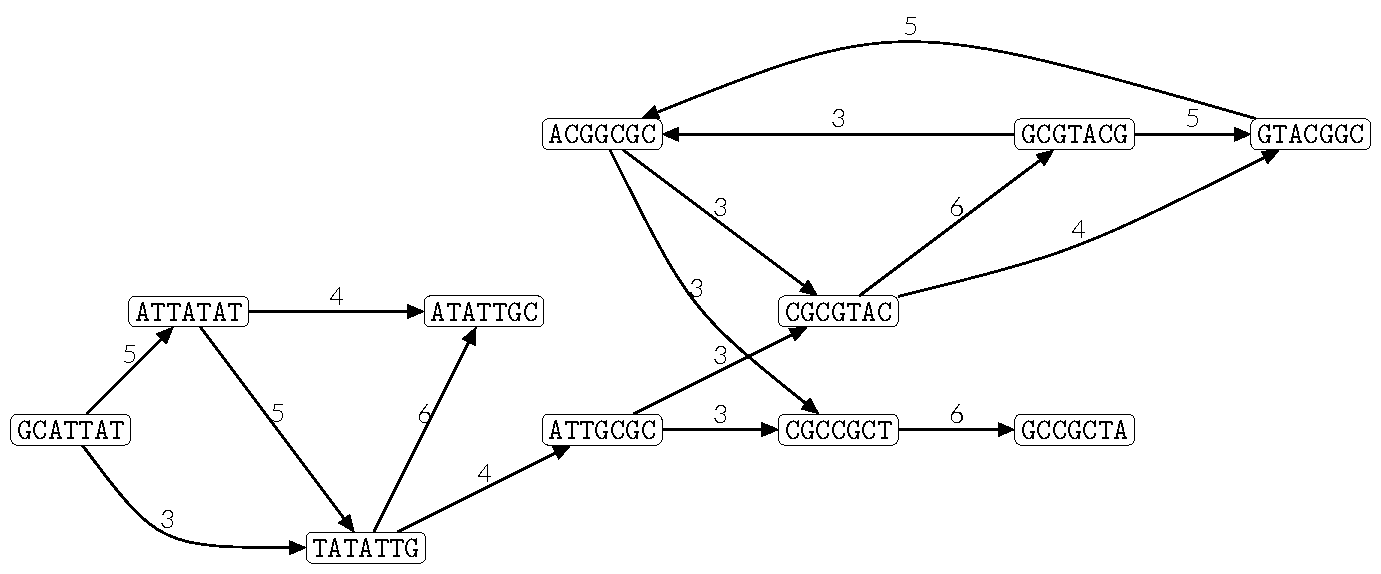
\includegraphics{fig-overlaps-dns-example}
% }}
% \caption{Sample overlap graph with each adjacent nodes 
% having at least $k = 3$ overlaps. The original string is \texttt{GCATTATATATTGCGCGTACGGCGCCGCTACA}.}
% \label{fig:dna-overlap}
% \end{figure*}	

% In \cite{Ma2009}'s paper, SCS was used to analyze DNA sequence assembly using
% a greedy algorithm. 

% \section{Project Context}

% \section{Purpose and Description}

% \section{Objectives}

% \vfill\eject
\section{Scope and Limitations}
The researchers will utilize Haskell for concrete implementation 
of the parallel A* algorithm in a functional programming environment.
Likewise, for performance comparison, the researchers 
will use the Rust programming language due to some of its features having
similarities with Haskell such as correct concurrent programs\cite{Saligrama2019}
and guarantees a relatively safe program\cite{Jung2018}.

Other purely-functional languages or lambda notation for generality
will not be used. Other concurrent data structures besides \verb|MVar| and Software
Transactional Memory will not be utilized.
%%%%%%%%%%%%%%%%%%%%%%%%%%%%%%%%%%%%%%%%%%%%%%%%%%%%%%%%%%%%%%%%%%%%%%%%%%%
\chapter{Review of Related Systems and Related Literature}
%%%%%%%%%%%%%%%%%%%%%%%%%%%%%%%%%%%%%%%%%%%%%%%%%%%%%%%%%%%%%%%%%%%%%%%%%%%

Due to the trend of parallelization in the modern computing era, \cite{Rios2011,WeinstockHolladay,ZaghloulAlJami2017,Sanz2016}
several researchers developed more efficient and faster implementations 
of the A* algorithm by parallizing the algorithm in various ways.

\section{The A* Algorithm}
The A* pathfinding algorithm, first described by Hart, Nilsson, and Raphael, is a \emph{best-first search} algorithm 
for finding a path between two vertices in a directed weighted graph.\cite{HartNilssonRaphael1968}
The A* search algorithm can be seen as a variant of Dijkstra's algorithm with an added heuristic function to guide its search 
for an optimal solution. That is, the A* search functions the same as Dijkstra's algorithm if the heuristic function $h(n)=0$
for any $n$.\cite{Ferguson2005} 

Hart, Nilsson, and Raphael had proven that the A* algorithm is \emph{admissible} whenever the heuristic
function $h$ is admissibe. That is, A* is guaranteed to return an optimal solution.
The optimality of the path generated by the A* algorithm depends on its heuristic function which will be discussed further in 
Chapter 3 of this paper. 
% Here, we shall describe the original A* algorithm by Hart, Nilsson, and Raphael.\cite{HartNilssonRaphael1968}
% A pure-function pseudocode\ref{seqAStar} will be implemented instead of the usual imperative 
% pseudocode. But the pseudocode still follows the specifications of the original paper.

% \begin{algorithm}
%     \caption{Sequential A* Algorithm}
%     \label{seqAStar}
%     \begin{algorithmic}
%         \REQUIRE $G$ - a weighted labeled graph.
%         \REQUIRE $(\psi, \xi)$ - a tuple of two sets: the open set and the closed set
%         \REQUIRE $h$ - the heuristic function. $h(n)\neq 0$ or this equates to Dijkstra's Algorithm.
%         \REQUIRE $(\sigma, \gamma)$ - a tuple of two vertices in $G$: the start vertex and end vertex.
%         \ENSURE  $p$ - The shortest path from $\psi$ to $\xi$. 
        
%         \STATE let $S$ be a homogenous set of vertices in a graph.
%         \STATE astar :: Graph $\rightarrow$ ($S$, $S$) $\rightarrow$ ((Int, Int) 
%             $\rightarrow$ (Int, Int) $\rightarrow$ Int) $\rightarrow$ (Vertex, Vertex) $\rightarrow$ Path 
%         \STATE astar g s h se p = \textbf{WRITE THE ALGORITHM LATER}.
%     \end{algorithmic}
% \end{algorithm}

% \begin{algorithm}[H]
% 	\begin{algorithmic}[1]
% 	\REQUIRE $R$ - set of strings
% 	\ENSURE superstring of set $R$
% 	\WHILE{||$R$|| > 1}
% 		\STATE choose $x_1 \neq x_2 \in R$ such that $overlap(x_1,x_2)$ is maximal 
% 		\STATE $R \leftarrow (R - \{x_1, x_2\}) \cup \{merge(x_1, x_2)\}$
% 	\ENDWHILE
% 	\RETURN remaining string in $R$
% 	\end{algorithmic}
% 	\caption{GREEDY(R)}
% 	\label{alg:seq}
% \end{algorithm}

\section{Parallel A* Algorithm}
Zaghloul, Al-Jami, Bakalla, et al. had shown that an implementation of a parallel A* algorithm 
had a speed up of 3-4 times on problem sizes of 2000x2000 to 4000x4000.\cite{ZaghloulAlJami2017}
The implementation took advantage of reducing the problem into subgraphs where the neighbors of a
vertex in a graph will have threads assigned to them and a neighbor $n_i$ will be the new start 
vertex of the A* search for that given thread with the same goal vertex. By Ahmdal's Law, 
runtime efficiency will decrease when the number of threads are increased due to the overhead 
of garbage collection and thread creation. 

\subsection{Bidirectional A* Search Algorithms}
Bidirectional search is said to be possible when there is exactly one start vertex and exactly one goal vertex.
Since the computer cannot differentiate between the two if they are reversible, it is possible to start 
searching from the goal $g$ to the start $s$ and vice versa.\cite{KainlKainz1997} Bidirectional search 
is useful when implemented on a unidirectional multigraph(\ref{uni-multigraph1})
where there can be an efficient path between from 
one vertex to another in one direction but the same path cannot exist in the other direction.

The BHPA algorithm is a bidirectional search employing two A* algorithms running sequentially with a sequential 
computer switching directions multiple times. The BHPA algorithm terminates whenever two search paths from both directions 
meet and returns the minimum $f$ cost of either direction or by adding the $g$ costs of the two directions.
However, Kaindl and Kainz had proven that the best case performance of BHPA* is not significantly better than 
the unidirectional A* algorithm due to the cost of the BHPA's termination condition.\cite{KainlKainz1997}
Kaindl and Kainz developed a more efficient implementation of a non-tradition bidirectional heuristic search that is effective 
on machines with limited memory. The algorithm instantiates by assigning memory to a unidirectional approach and uses A* to find 
a path from the start to the end vertices. If there is such a path given the memory, then the algorithm terminates. Otherwise, 
a reverse search from the end vertex to an intermediate vertex from the first search.

The New Bidirectional A* Search (NBA*) uses the same technique as the BHPA in the sense that the execution of each search direction alternates.\cite{Pijls2009}
However, NBA* employs the reverse search on a reverse graph. That is, let $V(G)$ and $E(G)$ be the vertex set and edge set of graph $G$ and if $u,v\in V(G)$ and 
$uv\in E(G)$ but $vu\notin E(G)$, then for the reverse graph $\text{rev}(G)$ with $u,v\in V(\text{rev}(G))$ and $vu\in E(\text{rev}(G))$ but $uv\notin E(\text{rev}(G))$.
The edges $uv$ in $E(G)$ and $vu$ in $E(\text{rev}(G))$ have the same weights. Likewise, if $s_1$ and $t_1$ are the start and goal vertices of 
graph $G$, then $s_2$ and $t_2$ are the start and goal vertices of graph $\text{rev}(G)$ with $s_2=t_1$ and $t_2=s_1$. As a corollary, the vertex set of $\text{rev}(G)$
is equal to the vertex set of $G$ denoted by $V$ from this point.

In NBA*, all vertices $v\in V$ are initially labeled $g(v)=\infty$ and the set $\mathcal{S}=\varnothing$ is the set of vertices with
permanent labels. Likewise, there are shared variables $\mathcal{L}=\infty$ and $\mathcal{R}=\varnothing$ which will hold the the 
best cost so far and the rejected vertices, respectively. During the runtime of the algorithm, a vertex is either expanded if its heuristics 
or label satisfies the necessary conditions with respect to $\mathcal{L}$ or rejected and thus added in the set $\mathcal{R}$.
The algorithm halts when there is one search side with no more candidates to be expanded.



    \begin{figure}
        \caption{A directional multigraph}
        \label{uni-multigraph1}
        \begin{center}
            \begin{tikzpicture}
                \begin{scope}[every node/.style={circle,thick,draw}]
                    \node (A) at (0,0) {A};
                    \node (B) at (4,0) {B};
                    \node (C) at (7,3) {C};
                    \node (D) at (7,-3) {D};
                    \node (E) at (10,0) {E};
                \end{scope}
                
                \begin{scope}[>={Stealth[black]},
                              every node/.style={fill=white,circle},
                              every edge/.style={draw=red,very thick}]
                    \path [->] (A) edge[bend left=30] node {$5$} (B);
                    \path [->] (B) edge[bend right=-30] node {$5$} (A);
                    
                    \path [->] (B) edge[bend left=30] node {$10$} (C);
                    \path [->] (C) edge[bend right=-30] node {$10$} (B);
                    \path [->] (D) edge node {$7$} (B);
    
                    \path [->] (E) edge[bend left=30] node {$3$} (D);
                    \path [->] (D) edge[bend right=-30] node {$4$} (E);
                    \path [->] (C) edge[bend left=30] node {$5$} (E);
                    \path [->] (E) edge[bend right=-30] node {$10$} (C);

                \end{scope}
            \end{tikzpicture} 
        \end{center}
        
    \end{figure}

\subsubsection{Parallel New Bidirectional A* (PNBA*)}
PNBA* was proposed by Rios and Chaimowicz by parallelizing the NBA* algorithm.\cite{Rios2011}
PNBA* leverages on a shared memory model and runs both search processes in parallel. Due to this, the PNBA* algorithm is 
faster than the NBA* and thus has a better runtime performance. The implementation of PNBA* has a variable $\mathcal{S}$, like the 
NBA*, shared by both processes and contains the vertices, say $v$, with finite labels $g(v)$. However, since both $\mathcal{L}$
and $\mathcal{S}$ are updated by both processes in parallel, it is possible that there would be a race condition and some vertex 
in one thread may be expanded due to the race conditions. However, this does not affect the admissibility of PNBA*.
While this may incur some overhead due to expanding additional vertices, parallelism makes up for the additional overhead costs.\cite{Rios2011}

\subsection{Parallelism by Hashing}
The Hash Distributed A* Algorithm (HDA*) builds on the the hash-based work distribution of PRA* and asynchronous communication
by TDA.\cite{Kishimoto2009,Evett1995,Romein1999} The HDA* search introduces \emph{ownership} where each processor has their own local 
closed and open lists and the search space is divided among processors. Unlike the implementation by Zaghloul, when a vertex is expanded 
by a processor $P_1$ in HDA*, $P_1$ will not immediately own the generated vertices but instead send those vertices to the message queue 
to be hashed by available processors which can then be processed. A pseudo-random hash function is important to make sure work is distributed 
equally among available processors. If the hash function is static, that is it only assigns every generated vertex to the same processor that 
generated said vertices, then the algorithms performs the same way as the classic A* algorithm. Due to the parallel nature of HDA* and having 
local open and closed sets per processor, there is no guarantee that an expanded vertex will no longer be expanded.

The simplest approach for the termination condition of HDA* is the \emph{barrier method} wherein a processor waits for other processors 
when its open set is empty. This incurs some overhead and is not viable. Weinstock and Holladay describes the \emph{sum flags method} where a 
binary flag is raised by a processor if its open set is empty.\cite{WeinstockHolladay} Let $p_i$ be processors for all $i\in {1..n}$ where $n$ is the number of processors 
in the computer. The algorithm will terminate if $p_1\land p_2\land\dots\land p_n=True$.

The original paper by Kishimoto, Fukunaga, and Botea showed that HDA* performs significantly better than A*,
WSA*\footnote{Another parallel implementation of the A* algorithm that involves work stealing}, and PRA* when using message passing 
on a number of problems. When the HDA* is run using 4 CPU cores, the speedup averages 3 times and is shown to be very efficient 
compared to the other parallel implementations and the sequential A* algorithm. Likewise, the speedup is even more significant at 
an average of 5 times when using 8 cores. Kishimoto, Fukunaga, and Botea expounded further that the HDA* is also efficient in a 
distributed computing environment by showing a speedup of an average of 30-60 times in a 128-core distributed computer.\cite{Kishimoto2009}

\section{Real-time Performance of Functional Programs}
The dominant programming languages used for time-critical software systems such as GPS systems and flight guidance softwares 
are written in mid-level programming languages that has direct hardware access such as C or C++. Frame and Coffey were concerned that 
the correctness of C and C++ were refutable and thus benchmarked and compared the real-time performance of the same 
program written in C++ and in Haskell, the latter being a programming language known to its correctness due to its strict typing rules.\cite{Frame2014}
Frame and Coffey hypothesized that imperative and functional programming may differ in their implementations but both are powerful enough to 
take on math-intensive problems.

Scott and Frame also tacked the ease of use of the programming language to the programmers and they concluded that 
the functional programming language may seem unfamiliar to an imperative language user at first but may be easier to 
understand and maintain in the long run.\cite{Frame2014} This is especially true in static typing languages such as Haskell 
where programmers will be able to make less typing errors such as adding a \verb|uint_8| to a \verb|bool| which may cause an overflow.\cite{Hanenberg2014}
The paper by Scott and Frame showed that functional programs are less verbose and are more expressive than their imperative counterparts 
for the same problem, however it still lacks in performance power. However, despite the slower runtime performance of functional programs, mathematically 
provable functional programs are still capable in being written as runtime verification systems in ultra-critical systems, as 
demonstrated by the National Aeronautics and Space Administration (NASA).\cite{NasaCopilot2020} Due to this, it is 
important to develop more performant, perhaps parallel, algorithms for functional programs especially in the area of 
combinatorial optimization, such as the problem posed in this paper.

Harris, Marlow, and Jones evaluated the parallel performance of Haskell and overhead costs when using parallel data structures.
Since Haskell is a garbage collected programming language, there would be some performance cost whenever data is being garbage collected.
However, due to the lazy-nature of Haskell, unecessary data that will never be used in any computation will not be evaluated.
The parallel impleentation of the Glasgow Haskell Compiler (GHC) does not really state explicit parallelism. Instead, a programmer may 
annotate (called \emph{sparking}) whether a computation can be parallelized or not with different strategies. 
It is up to the Haskell runtime system whether the annotation will be assigned to a different processor or thread. 
This abstraction enables the programmer to be worry-free about how parallelism will be implemented and diverts it to 
other matters such as performance and how many sparks will be created.\cite{Harris2005,Marlow2009} 
% Several researches have provided in depth study on approximation
% algorithms for the SCS problem.

% Most \cite{Turner1989, Ma2009, Zaritsky2004}, however, considered a greedy algorithm to solve the SCS problem.
% The reason why greed works for shortest common superstring problem was
% explored by \cite{Ma2009}. They explained the good performance 
% of the greedy algorithm by using the smoothed analysis. 
% That is, for any  given instance $I$ of $SCS$, 
% the average approximation ratio of the 
% greedy algorithm on a small random perturbation of $I$ is $1+o(1)$. 

% Apart from the greedy approach, other methods including bio-inspired
% algorithms, have also been employed to solve lots of hard problems in 
% computer science including the SCS problem. 
% In \cite{Zaritsky2004}'s work, for example, four approaches for 
% finding solutions to the SCS problem: a 
% standard genetic algorithm, a novel cooperative-coevolutionary 
% algorithm, a benchmark greedy algorithm, and a parallel 
% coevolutionary-greedy approach have been compared. In the paper,
% the coevolutionary approach produced the best results.

% Zaritsky et al's \cite{Zaritsky2004} work served as the 
% foundation of this paper. Hence, the following algorithms,
% which have been explored and tested in the latter, have
% been extracted and validated 
% whether they are indeed generating
% good approximate solution to the SCS problem.

% \subsection{Greedy-SCS}

% The core idea of the greedy algorithm is to repeatedly merge
%  pairs of distinct strings with maximum overlap until only one remains.
%  It has been conjectured by \cite{MaierStorer1777} that the superstring
%  produced by the greedy algorithm is at most two times the optimal.
% Below is a pseudocode for the greedy algorithm:

% \begin{algorithm}[H]
% 	\begin{algorithmic}[1]
% 	\REQUIRE $R$ - set of strings
% 	\ENSURE superstring of set $R$
% 	\WHILE{||$R$|| > 1}
% 		\STATE choose $x_1 \neq x_2 \in R$ such that $overlap(x_1,x_2)$ is maximal 
% 		\STATE $R \leftarrow (R - \{x_1, x_2\}) \cup \{merge(x_1, x_2)\}$
% 	\ENDWHILE
% 	\RETURN remaining string in $R$
% 	\end{algorithmic}
% 	\caption{GREEDY(R)}
% 	\label{alg:seq}
% \end{algorithm}

% The greedy algorithm is probably the most widely used
% heuristic used in DNA-sequencing due to its simplicity and 
% constant performance guarantee which is most likely to be factor-2.

% \subsection{Genetic Algorithm}

% In this paper, we follow the standard model for the genetic algorithm (see Algorithm \ref{alg:gga}).
% That is, the algorithm generates an initial population of 
% random candidate solutions, then 
% the process of selection based on a defined fitness function,
% crossover, and mutation are used to evolve the next generation, of which
% each individual is then evaluated and
% assigned a fitness value. These steps are repeated a
% predefined number of times or until the solution is
% satisfactory. 


% \begin{algorithm}[H]
% 	\begin{algorithmic}[1]
% 	\STATE $t \leftarrow 0$ \{generation number\} 
% 	\STATE initialize Population$_{t}$ 
% 	\STATE evaluate(Population$_{t}$)
% 	\WHILE{termination condition not met}
% 		\STATE select individuals from Population$_{t}$ 
% 		\STATE recombine individuals
% 		\STATE mutate individuals	
% 		\STATE Population$_{t+1} \leftarrow $ newly created individuals
% 		\STATE $t \leftarrow t + 1$
% 		\STATE evaluate(Population$_{t}$) 			
% 	\ENDWHILE
% 	\RETURN solution derived from the best individual in Population$_{t}$
% 	\end{algorithmic}
% 	\caption{GENERIC GA()}
% 	\label{alg:gga}
% \end{algorithm}

%%%%%%%%%%%%%%%%%%%%%%%%%%%%%%%%%%%%%%%%%%%%%%%%%%%%%%%%%%%%%%%%%%%%%%%%%%%%
\chapter{Technical Background}
%%%%%%%%%%%%%%%%%%%%%%%%%%%%%%%%%%%%%%%%%%%%%%%%%%%%%%%%%%%%%%%%%%%%%%%%%%%

\section{Graph Theoretic Preliminaries}
A weighted, directed graph $G=(V,E)$ with $V$ being the set of vertices of $G$ and $E$ being the set 
of edges of $G$ is said to be a graph with an associated weight function $w:E\to\mathbb{R}$ mapping the edges of $G$
to real-valued weights. The $\walk{u}{v}$, where $u,v\in V$ is a sequence of vertices $(u, u_1, u_2,\dots,v)$ where 
consecutive vertices are adjacent to each other in $G$. A $\graphpath{u}{v}$ is a $\walk{u}{v}$ with no repeating vertices,
implicitly, no repeating edges.

In this paper, an edge is denoted by the two vertices incident of the edge. Example, for two vertices $u$, $v$ in a graph, 
an edge between $u$ and $v$ would be denoted by $uv$. Hence, a path $(v_0, v_1, \dots, v_n)$ has edges
$\{v_0v_1, v_1v_2,\dots, v_{n-1}v_n\}$. 

\section{Minimum Cost Paths}
The minimum cost paths is a discrete optimization problem wherein the goal is to determine 
the shortest path from a start vertex in a graph to an end vertex in a graph. This paper only 
deals with single-source shortest path. The shortest path problem can be defined formally as follows.

The function $W$ of a path $W(p)$ where $p$ is a path is denoted by the sum of the edges 
in the path.\cite{CLRS} That is, if some path $p=(v_0, v_1, \dots, v_n)$, the function $W$ is defined as 
\[
W(p) = \sum^k_{i=1} w(v_{i-1}v_i). 
\]

Hence, the shortest path weight can be defined by the function $\zeta: V\to V$ (a mapping from a vertex in $G$ to another vertex in $G$)
as follows 
\[
\zeta(u, v)=\begin{cases}
    \text{min}(S_{u\to v}) & \text{if there is a path from $u$ to $v$} \\ 
    \infty  & \text{otherwise}
\end{cases}    
\]
where $S_{u\to v}$ is the set of weights of all paths from $u$ to $v$, that is, $S_{u\to v}=\{W(p) | p=(u,v_1, v_2,\dots, v)\}$.
Hence, the \textbf{shortest path} is defined as the path with the shortest weight, that is $W(p)=\zeta(u, v)$.\cite{CLRS}

\section{A* Algorithm}
While the shortest path in a graph problem can be solved by dynamic programming, other algorithms exist such as branch and bounding algorithms 
like the A* search.\cite{HartNilssonRaphael1968} The A* search algorithm employs the use of heuristic functions to estimate the cost
or distance from the current vertex to the final vertex, while keeping in mind the current best. Hence, the A* search can be thought of 
as an intelligent algorithm in the classical sense. A heuristic function is \textbf{admissible} if it is proven that it will never 
overestimate the cost of reaching the end vertex. That is, the heuristic function may underestimate or equal the actual cost. 
Assuming the heuristic function is admissible, then the A* algorithm is considered to be admissible. 

Likewise, the heuristic function of the A* algorithm is \textbf{consistent} or monotone if the estimate of the cost from the current 
vertex is always less than or equal to the cost of its neighbors in the open set (vertices that haven't been analyzed) to the end vertex
plus the cost of reaching the neighbor from the current vertex.

\begin{definition}
    If a vertex $v$ is in the closed set, then it is \textbf{expanded}. Likewise, \textbf{expanding} $v$ means adding $v$ to the closed set.
\end{definition}

\begin{algorithm}[H]
    \begin{algorithmic}[1]
        \REQUIRE $G$ - the graph
        \REQUIRE $u$ - start vertex.
        \REQUIRE $v$ - end vertex 
        \STATE Let $\Omega$ be the open set.
        \STATE Let $\Gamma$ be the closed set.
        \STATE Let $f$ be the evaluating function
        \STATE Add $u$ to $\Omega$.
        \WHILE {$\Omega\neq\varnothing$}
            \STATE Get the vertex $a\in\Omega$ with the minimum $f(a)$.
            \IF{$a=v$}
                \STATE Add $a$ to $\Gamma$ and terminate A* search.
            \ELSE 
                \STATE Add $a$ to $\Gamma$
                \STATE Let $N$ be the set of adjacent vertices of $a$ not in the closed set.
                \STATE For all $n\in N$, add $n$ to $\Omega$.
                \STATE For neighbors $m$ of $a$ in the closed set
                \IF {$f(m)$ is lower than the cost when $m$ is expanded}
                    \STATE Unexpand $m$, that is, add $m$ to the open set 
                \ENDIF
            \ENDIF
        \ENDWHILE
    \end{algorithmic}
    \caption{A* Search Algorithm}
\end{algorithm}

% \begin{algorithm}[H]
% 	\begin{algorithmic}[1]
% 	\REQUIRE $R$ - set of strings
% 	\ENSURE superstring of set $R$
% 	\WHILE{||$R$|| > 1}
% 		\STATE choose $x_1 \neq x_2 \in R$ such that $overlap(x_1,x_2)$ is maximal 
% 		\STATE $R \leftarrow (R - \{x_1, x_2\}) \cup \{merge(x_1, x_2)\}$
% 	\ENDWHILE
% 	\RETURN remaining string in $R$
% 	\end{algorithmic}
% 	\caption{GREEDY(R)}
% 	\label{alg:seq}
% \end{algorithm}

\section{Parallel A* Algorithm}
Two parallel methods described will be used in this paper. Specifically, HDA* and PNBA*.\cite{Kishimoto2009,Rios2011}

\subsection{PNBA*}
The PNBA* is a parallelization of the bidirection A* algorithm. One of the main advantages of computing the shortest path 
bidirectionally is that it reduces the search space and search effort.\cite{KainlKainz1997,Pijls2009}. The execution of the PNBA*
can be done on a computer with two CPU cores (or two CPUs). One CPU searches forwardly, that is, from the start vertex, it finds a 
path to the end vertex. The other CPU searches backwardly wherein it starts from the end vertex to the start vertex. The PNBA* heuristic function 
need not impose that the used heuristic function is admissible. That is, only consistency is needed. As discussed in Chapter 2, the PNBA* is a 
parallelized version of the NBA*. Since the NBA* employs alternating execution between the two directions, it may be distributed on two different 
CPU cores as demonstrated by Rios and Chaimowicz. The PNBA* can use a data structure such as a priority queue. Each direction will have their own 
priority queue to serve as the open set $\Omega_p$ for $p\in\{1,2\}$, for each process $p$, as stated in the paper by Rios and Chaimowicz.

\begin{definition}
    A vertex $v$ is \textbf{labeled} if the estimate $g(v)$ (the shortest path found so far, that is, an estimate of $\zeta(v_{start}, v)$)
    is finite and $v$ hasn't been expanded.
\end{definition}

The paper establishes the following notational convention to be used for the rest of the paper with regards to the PNBA* algorithm. 
Two processes exist, namely process $p$ in $p\in\{1,2\}$. Whenever $p$ is used, it is implied that $p$ is the process number, i.e the CPU being 
referenced. Let $h_p(v)=\zeta_p(v, v_{goal})$ be the heuristic for estimating the cost from the current vertex $v$ to the goal vertex $v_{goal}$.
Likewise, let $g_p(v)=\zeta_p(v_{start}, v)$ be shortest path so far. The shared set $\mathcal{M}$ contains the vertices in the middle of the two searches.
Initially, all vertices are in $\mathcal{M}$. The shared variable $\mathcal{L}$, the best solution so far, initially set to $\infty$ since 
the algorithm will need to minimize $\mathcal{L}$ as small as possible. The variable $F_p$ is the lowest $f_p$-value of $\Omega_p$ where $f_p(v)=h_p(v)+g_p(v)$.
The variables $f_p$, $g_p$, and $F_p$ can be written only by process $p$ but can be read by both. Note that it is best to implement the open sets $\Omega_p$.

Though an abuse of notation, if $p\in\{1,2\}$ then $\neg:\{1,2\}\to\{1,2\}$ is described as follows:
$$
\neg p=\begin{cases}
    1 & \text{if } p=2 \\ 
    2 & \text{if } p = 1.
\end{cases}
$$

\begin{algorithm}[H]
    \caption{PNBA* (Parallel New Bidirectional A*) Search Algorithm}
    \begin{algorithmic}
        \REQUIRE $G$, the graph 
        \REQUIRE $u$, start vertex and $v$, the end vertex
        \STATE Let $\mathcal{M}$ contain all vertices in $G$ and for all $m\in\mathcal{M}$, let $g_p(m)=\infty$.
        \STATE Let $s_1=t_2=u$ and $s_2=t_1=v$.
        \STATE Set $g_p(s_p) = 0$ and add $s_p$ into $\Omega_p$.
        \STATE From here on, all instructions are run in parallel.
        \WHILE {$\Omega_1\neq\varnothing$ or $\Omega_2\neq\varnothing$}
            \STATE Get the vertex $n\in\Omega_p$ with the minimum $f_p(n)$.
            \IF {$n\in\mathcal{M}$}
                \IF {$f_p(n)<\mathcal{L}$ and $g_p(n)+F_{\neg p}-h_p(n)<\mathcal{L}$}
                    \FORALL {$m$ is a neighbor of $n$ and $m$ is not expanded}
                        \IF {$m\in\mathcal{M}$ and $g_p(m)>g_p(n)+\zeta_p(nm)$}
                            \STATE Set $g_p(m)=g_p(n)+\zeta_p(nm)$
                            \STATE Set $f_p(m)=g_p(m)+h_p(m)$
                            \IF {$m\in\Omega_p$}
                                \STATE Remove $m$ from $\Omega_p$ 
                            \ENDIF
                            \STATE Insert $m$ to $\Omega_p$.
                            \IF {$g_1(m)+g_2(m)<\mathcal{L}$}
                                \STATE Lock $\mathcal{L}$ to ensure that $F_p$ and $L$ are monotonic.
                                \IF {$g_1(m)+g_2(m)<\mathcal{L}$}
                                    \STATE Set $\mathcal{L}=g_1(m)+g_2(m)$.
                                \ENDIF
                                \STATE Unlock $\mathcal{L}$ after the update.
                            \ENDIF
                        \ENDIF
                    \ENDFOR
                \ENDIF
                \STATE Remove vertex $n$ from $\mathcal{M}$.
            \ENDIF
            \IF {$\Omega_p\neq\varnothing$}
                \STATE Set $F_p$ with the lowest $f_p$-value in $\Omega_p$.
            \ENDIF
        \ENDWHILE
    \end{algorithmic}
\end{algorithm}

\subsection{HDA*}
Unlike the PNBA*, the Hash-Distributed A* Search can employ the use of as many CPU cores as desired.\cite{Kishimoto2009} One 
of the main advantages of this is that it can easily be implemented on a GPU with hundreds or thousands of cores, thereby, 
execution would be faster. In the PNBA*, each process has different closed and open sets but in the HDA*, 
these sets are a parallel data structure shared among each CPU cores. However, there is a hash function $k:V(G)\to P$ where 
$V(G)$ is the set of vertices in $G$ and $P$ is the set of processors. When a new vertex is found and the hash function is computed for 
the vertex, the algorithm determines which CPU core should own the vertex based on the hash function.\footnote{Like how a hashmap works}
Thereby, while the open and closed sets are implemented as a parallel data structure, each processor owns a space 
in the open and closed set denoted by $\Omega_p$ and $\Gamma_p$ respectively for processor $p$, based on the hash key.

\begin{algorithm}[H]
    \caption{HDA* (Hash-Distributed A*) Search Algorithm}
    \begin{algorithmic}
        \REQUIRE $G$, the graph 
        \REQUIRE $u$, the start vertex 
        \REQUIRE $v$, the goal vertex
        \STATE Let $\Omega$ be the open set and $\Gamma$ be the closed set. Let $f$ be the evaluating function.
        \STATE Add $u$ to $\Omega$
        \STATE Everything from here on is run in parallel. Each processor $p$ runs the while loop below.
        \WHILE {global $\Omega\neq\varnothing$}
            \IF {$p$ has a new vertex $a$ in its message queue.}
                \IF {$a\notin\Gamma_p$}
                    \STATE Add $a$ to $\Omega_p$.
                \ENDIF
            \ELSE
                \STATE Get the vertex $a$ with the minimum $f(a)$ from $\Omega_p$.
                \STATE Let $N$ be the set of neighbors of $a$ not in $\Gamma_p$.
                \STATE Compute hash key $k(n)$ for all $n\in N$
                \STATE Let $p'$ be the processor that owns the hash key $k(n)$.
                \WHILE {The message queue of $p'$ is locked by another processor}
                    \STATE Wait
                \ENDWHILE
                \STATE Lock $p'$ message queue
                \STATE Send $n$ to $p'$
                \STATE Unlock $'$ message queue.       
            \ENDIF
        \ENDWHILE
    \end{algorithmic}
\end{algorithm}

\section{Haskell Parallel Runtime}
Haskell's parallel execution is implicit and can be done in a monadic environment.\cite{Marlow2013}
Since Haskell is a functional program, the task of parallelization is made easy by the runtime 
by \lstinline{rpar} and \lstinline{rseq} and by specifying strategies on how haskell should 
parallelize the task. However, the Glasgow Haskell Compiler (GHC) runtime may or may not parallelize 
the function at all, this is because \lstinline{rpar} sparks the function for parallelization, that is,
there is a potential that it may be parallelized.\cite{Marlow2005} A common problem for parallelization 
in Haskell is that the runtime garbage collection might take more time compared to the actual algorithm 
execution, therefore decreasing efficiency significantly. This can be mitigated and prevented by analyzing 
the granularity of the data structures. For example,
\begin{lstlisting}[language=Haskell]
    -- We have a list of 10000 elements
    xs = [0..10000]
    -- square all elements of xs
    xs' = (^2) <$> xs
    -- execute in parallel
    runEval (evalList xs')
\end{lstlisting}
This example is inefficient since the GHC runtime will assign each element of \lstinline{xs} to a different 
thread, thereby increasing CPU overhead and garbage collection since the inexpensive task of squaring 
numbers is undermined by the more expensive task of garbage collection. A better implementation would be 
\begin{lstlisting}[language=Haskell]
    -- We have a list of 10000 elements
    xs = [0..10000]
    -- square all elements of xs
    xs' = (^2) <$> xs
    -- execute in parallel
    runEval (parListChunk 5000 xs')
\end{lstlisting}
In this example, the GHC runtime will divide the list into two and have two different processors 
evaluate the two sublists. This way, the processor assignment and garbage collection overhead will be minimized.

Hence, in Haskell, problems of parallelization switched from the implementation details such as deadlocks, 
race conditions, and others commonly encountered in other languages, to that of the dividing the task into 
chunks that GHC will be performant.

\section{Maze Generation}
The mazes were generated using Python and exported to a text file using Depth-First-Search algorithm.
Since the depth-first search algorithm is guaranteed to produce a solvable maze, the researchers chose to use 
depth-first search when generating the maze.

Two versions of the DFS algorithm were used. One of them were randomized node selection while exploring the grid.
The second was to choose randomly whether the selected node will remain open, that is, have no wall, or to be closed.
The randomization of the DFS algorithm will generate a more robust and unpredicted maze generation that ensures 
there are multiple ways to solve a given maze.\cite{CLRS}

% Likewise, we discuss the graph representation we will use (adjacency list vs adjacency matrix)
% and how Haskell's parallelization works with respect to the Haskell Runtime, such as how 
% sparks are created which may or may not be parallelized at all! 

% We're still debating whether to use the Categorical Abstract Machine so there's no loss of generality 
% over different programming languages. If so, we will discuss a little bit of the syntax and notation for formality.
% If not, we will skip this step and proceed with using a concrete implementation of Haskell.

% Here, we discuss the original A* algorithm which is implemented in abstracted Haskell and two different parallel A* algorithm in 
% a Python-like pseudocode, specifically, PBA* and HDA*.
% A superstring is simply a string over
% some alphabet for which given a set of string from the same
% alphabet, the latter's members are all substrings of the former.
% To understand the SCS problem, it is best to assume some important concepts
% related to the problem itself. First, let
% us assume some set $R = \{x_1, \ldots , x_n\}$ as
%  a set of strings (or blocks) over some alphabet $\Sigma$. 
% Formally, we define a $superstring$ of $R$ as a 
% string $w$ containing each $x_i \in R$, as a substring.

% Following are the elementary operations associated 
% with the construction of a superstring.
% The $overlap(u, v)$ of two strings $u$ and $v$ 
% is the maximum overlap between $u$ and $v$. That is to say,
% the longest suffix of $u$ (in terms of characters) that is a prefix of $v$.
% The $prefix(u, v)$ of $u$ and $v$ is the prefix of $u$
% obtained by removing its overlap with $v$.
% Lastly, $merge(u, v)$ is the
%  concatenation of $u$ and $v$ with the overlap appearing
% only once.

% As an example, say we have, $\Sigma = \{a, b, c\}$ and $R = \{cbcaca, cacac\}$.
% The string $cacacbcaca$ is a superstring of $R$ while the string
% $cbcacac$ is the shortest common superstring. The
% following relations also hold: 

% \begin{tabular}{p{0.5cm}l}
% &$overlap(cbcaca, cacac) = caca$, \\
% &$overlap(cacac, cbcaca) = c$ ,\\
% &$prefix(cbcaca, cacac) = cb$,\\
% &$merge(cbcaca, cacac) = cbcacac$.
% \end{tabular}

% A $superstring$ $w$ is also defined as
%  the string $prefix(x_1, x_2) \cdot prefix(x_2, x_3) \cdots prefix(x_n, x_1) \cdot overlap(x_n, x_1)$.
% That is, a $superstring$ is simply
%  a concatenation of all the strings ``minus'' the overlapping duplicates.
%  Apparently, each superstring of a set of strings defines a permutation of the set’s elements.
% Conversely, every permutation of the set’s elements corresponds to a single superstring
			 
% Our interest however lies on defining the SCS problem.
% Essentially, the SCS problem is: Given a set of strings $R$
% and a positive integer $K$, does $R$ have a superstring of length $K$?

% Figure \ref{fig:scsdp} shows the SCS Decision Problem following the template
% provided by Garey and Johnson \cite{GareyJohnson1979}.

% \begin{figure}[ht!]
% \centering
% \fbox{
% \begin{tabular}{p{7.5cm}}

% INSTANCE: \\
% Finite alphabet $\Sigma$, finite set $R$ of strings from $\Sigma^*$ and a positive integer $K$. \\
% QUESTION: \\
% Is there a string $w \in \Sigma^*$ with $\vert w\vert \leq K$ such that each string $x\in R$ is a substring of w, 
% i.e. $w=w_0 x w_1$ where  $w_0,w_1\in\Sigma^*$? \\
% \end{tabular}
% }
% \caption{SCS Decision Problem }
% \label{fig:scsdp}
% \end{figure}


% In the Compendium of NP Optimization problems published by \cite{AusielloEtAl2000} and in the list of 
% NP-Complete Problems published by \cite{GareyJohnson1979} the SCS problem appears under under Storage and Retrieval (SR).
%%%%%%%%%%%%%%%%%%%%%%%%%%%%%%%%%%%%%%%%%%%%%%%%%%%%%%%%%%%%%%%%%%%%%%%%%%%%
\chapter{Methodology}
%%%%%%%%%%%%%%%%%%%%%%%%%%%%%%%%%%%%%%%%%%%%%%%%%%%%%%%%%%%%%%%%%%%%%%%%%%%

Methodology stuff will appear here.


\section{Systems Analysis}

\section{Systems Design}

\section{Requirements Specification}

\section{Development and Testing}

%%%%%%%%%%%%%%%%%%%%%%%%%%%%%%%%%%%%%%%%%%%%%%%%%%%%%%%%%%%%%%%%%%%%%%%%%%%%
\chapter{Results}
%%%%%%%%%%%%%%%%%%%%%%%%%%%%%%%%%%%%%%%%%%%%%%%%%%%%%%%%%%%%%%%%%%%%%%%%%%%

The researcher conducted an experiment to validate the results
in \cite{Zaritsky2004}'s work. Following is the description of the 
experiment done.

The input strings used in the experiment were generated in a
 manner similar to the one used in DNA sequencing. That is, a random
string is generated, duplicated a predetermined number of times,
 and the copies are randomly divided into blocks of a given size. 
 The set of all these blocks is the input to the SCS problem. 
 The reasons for choosing this type of input has been extensively
 explained in \cite{Zaritsky2004}.
Since our random string is a sequence of characters \texttt{A},\texttt{C},\texttt{G}, and \texttt{T}, we must 
transform this into an equivalent binary string. To do this, we simply 
assign each letter a unique two-bit representation, that is, 
\texttt{A = 00}, \texttt{C = 01}, \texttt{G = 11}, and \texttt{T = 10}. 

The parameters used in the input generation is as follows:

\begin{tabular}{p{0.5cm}l}
&\textit{Size of random string}: 250 bases or characters\\
&\textit{Minimal block size}: 20 characters\\
&\textit{Maximal block size}: 30 characters\\
&\textit{Number of duplicates created from the random string}: 5\\
\end{tabular}

Let $l$ denote the length of the derived string in the
genetic algorithm case. Let $m$
denote the number of blocks not covered by the derived string, 
and let $b$ denote the maximal block size
(30, in our case). The fitness value, $f$ , of an individual
is computed as follows:
\[f = \dfrac{1}{l + m*b}\] 
This fitness function above drives evolution towards
shorter superstrings covering as many blocks as possible.

We performed 50 randomly generated problem instances.
On each problem instance each type of genetic algorithm was executed
twice and the better run of the two was used for statistical purpose.
The results are summarized in Table \ref{tbl:resultsga} and is presented graphically in Figure \ref{fig-results}.


\begin{table}
\centering
\begin{tabular}{|c|c|c|}
\hline
Number  & Average Superstring  & Average  \\
 of& Length (Rounded to & Runtime \\
Generations& Nearest Units) & (in Seconds) \\
\hline
\hline
100		& 760	& 34.57		\\
250		& 596	& 74.20		\\
500		& 526	& 139.70	\\
1000	& 482	& 267.09	\\
5000	& 421	& 1038.73	\\
10000	& 413	& 1943.55	\\
20000	& 409	& 3700.57	\\
\hline
\end{tabular}
\caption{
Average superstring length and runtime of our Genetic Algorithm
on 50 randomly generated problem instances. Each input set contains
50 blocks.}
\label{tbl:resultsga}
\end{table}


\begin{figure*}[ht!]
\centering
\fbox{
\scalebox{0.55}{
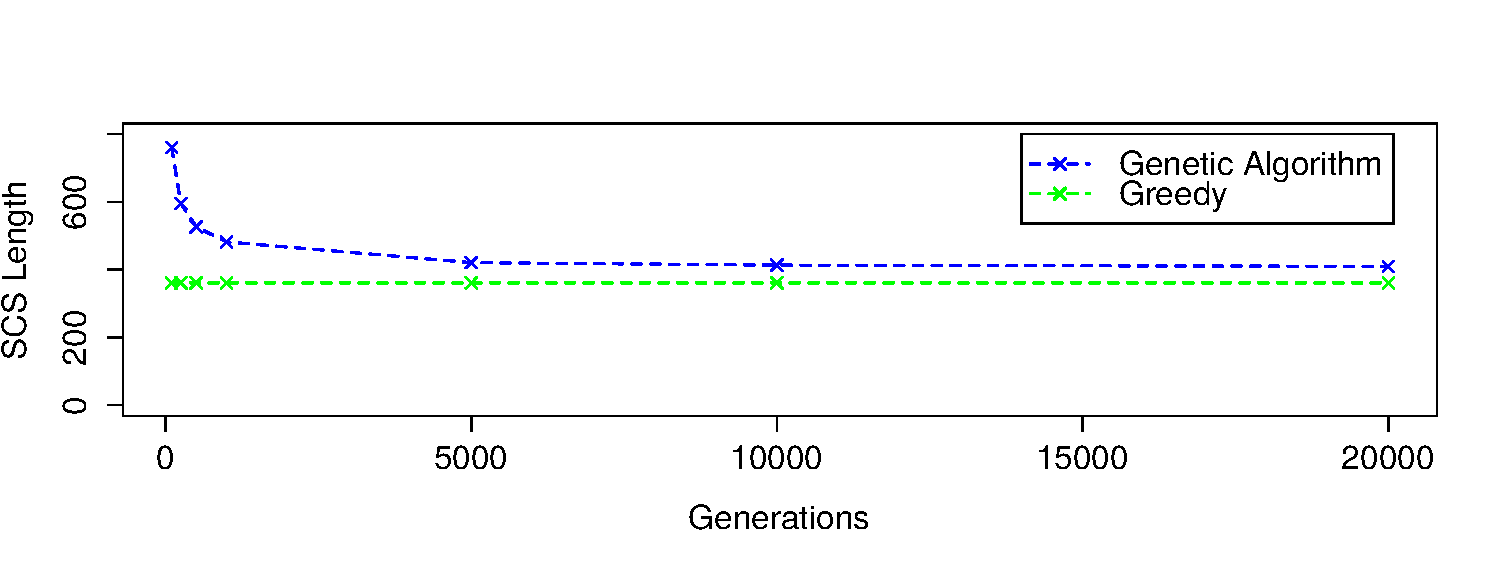
\includegraphics{result-gavsgreedy.pdf}
}}
\caption{Best superstring as a function of generations. Each point in the figure represents the average of 50
runs on 50 different randomly generated problem instances. For each such instance, two runs were performed, the better
of which was considered for statistical purposes}
\label{fig-results}
\end{figure*}

Note that our results seem to disagree with that of \cite{Zaritsky2004}.
In contrast with the latter's findings, our tests shows that
the greedy algorithm outperformed the genetic algorithm both in terms of finding superstrings
with minimal length and the the time it takes to do so.

On the same set of test cases, the greedy algorithm
produced superstrings having an average of 361 characters, 
in an average of runtime 130.64 milliseconds. This is far better than
the 409 average superstring length that the genetic algorithm
derived in 20000 generations in more or less an hour of operation. 
Note that the average length of the superstring derived by the greedy algorithm is
less than the conjectured factor-2 performance guarantee.
Recall that the length of the initial (reference) string is 250.

Still it is good to note that the genetic algorithm approach
in solving the SCS problem converges. That is, we see a better solution
yield as time or generations progress. 
%%%%%%%%%%%%%%%%%%%%%%%%%%%%%%%%%%%%%%%%%%%%%%%%%%%%%%%%%%%%%%%%%%%%%%%%%%%%
\chapter{Contributions and Recommendations}
%%%%%%%%%%%%%%%%%%%%%%%%%%%%%%%%%%%%%%%%%%%%%%%%%%%%%%%%%%%%%%%%%%%%%%%%%%%

\section{Summary of Contributions}


\section{Recommendations}


There could be several reasons why our tests did not yield the ``same'' results as that of \cite{Zaritsky2004}'s.
The author claims that this may be due to the myriad of parameters used in evolving
individuals in each step of the genetic algorithm and the large number of possible candidates or values that we can set these parameters with. 
For example, we may claim that the appropriate choice of the recombination technique is necessary. In \cite{Zaritsky2004},
a two-point crossover was employed. Thinking that this may be less of a factor, the author proceeded with just
one-point cross in implementing the genetic algorithm for the experiment.
Another could be in choice of the probabilities associated with recombination, elitism, and mutation rates.
The author did only consider what was stated in the base paper without performing tests to validate
whether this values are appropriate and could still complement the change made in some of the assumptions.
As such, more empirical tests could be done to appropriately estimate these parameters. 

If indeed DNA sequence assembly is the task at hand, lots of other techniques are now available.
One may consider for example representing the reads or DNA fragments in a de Bruijn graph
as opposed to the overlap graph presented in this paper. 
Assembling reads  in a de Bruijn graph 
reduces the problem to a fragment assembly problem that can be 
formulated as the goal to find a trail or Eularian path that visits 
each edge (read or fragment) in the (de Bruijn) graph exactly once. 
Such, somehow makes the assembly process much ``easier'' since Eularian path
construction is known to be solvable in deterministic polynomial time.



\appendix
% \chapter{Evaluation Tool}

Evaluation tool used goes here.

% \chapter{Sample Reports}

Describe and discuss the details of sample reports here.

% \chapter{Sample Input/Output}

Describe and discuss the details of sample I/O here.

\chapter{Code Listing}

%\lstinputlisting{src/scs-greedy.cpp}

% \chapter{User's Guide}




\nocite{*}
\bibliographystyle{siam}
{
\singlespace
\bibliography{references}
}

\begin{vita}
\verb|/*TODO*/| are BS Computer Science student of the
Department of Computer Science at the Ateneo de Naga University.
\end{vita}



\end{document}
